\documentclass[11pt,a4paper]{article}
\usepackage[T1]{fontenc}
\usepackage[margin=2.3cm]{geometry}
\usepackage{amsmath,amssymb,mathtools,booktabs,tabularx,array,enumitem,graphicx,float,caption,subcaption}
\usepackage[expansion=false]{microtype}
\usepackage{xcolor,colortbl,tikz,pgfplots,pgfplotstable,listings,fancyhdr,titlesec}
\usepackage{algorithm,algpseudocode}
\usetikzlibrary{arrows.meta,positioning,calc}
% Shared colours, plot styles and TikZ diagrams for slides.tex and report.tex.
\definecolor{ovgreen}{HTML}{138A07}
\definecolor{ovdark}{HTML}{0B5A04}
\definecolor{ovlight}{HTML}{E8F4E6}
\definecolor{ink}{HTML}{222222}
\definecolor{mute}{HTML}{6B6B6B}
\definecolor{today}{HTML}{E07B2A}
\definecolor{wait}{HTML}{7FBF6E}
\definecolor{late}{HTML}{C0392B}
\pgfplotsset{compat=1.18,
  fs axis/.style={axis lines=left, tick style={mute}, every axis label/.style={font=\footnotesize, color=mute},
    tick label style={font=\scriptsize, color=ink}, legend style={draw=none, font=\scriptsize, fill=none},
    axis line style={mute}, ymajorgrids, grid style={black!8}},
}
\tikzset{
  box/.style={draw=ovgreen, line width=.8pt, rounded corners=3pt, align=center, inner sep=6pt, fill=white},
  gbox/.style={box, fill=ovlight},
  arr/.style={-{Stealth[length=5pt]}, line width=.9pt, color=ovdark},
  pax/.style={circle, fill=today, minimum size=7pt, inner sep=0pt},
  lane/.style={draw=ovgreen, fill=ovlight, line width=.8pt, minimum width=1.25cm, minimum height=.55cm, rounded corners=2pt, font=\scriptsize},
}

% Single queue feeding c identical counters.
\newcommand{\queuediagram}{%
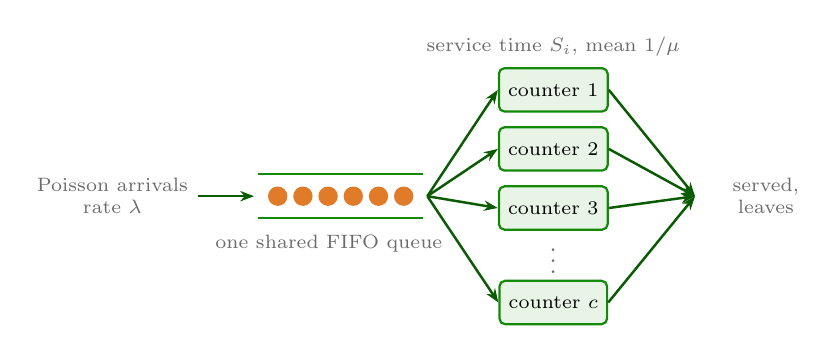
\begin{tikzpicture}[font=\small]
  \node[align=center, color=mute, font=\scriptsize] (src) at (0,0) {Poisson arrivals\\rate $\lambda$};
  \foreach \i in {0,...,5} \node[pax] at (2.1+\i*0.32, 0) {};
  \draw[ovgreen, line width=.8pt] (1.85,-.28) -- (3.95,-.28) (1.85,.28) -- (3.95,.28);
  \node[font=\scriptsize, color=mute] at (2.75,-.6) {one shared FIFO queue};
  \draw[arr] (src.east) -- (1.8,0);
  \foreach \k/\y in {1/1.35, 2/.6, 3/-.15, c/-1.35} {
    \node[lane] (l\k) at (5.6,\y) {counter $\k$};
    \draw[arr] (4.0,0) -- (l\k.west);
    \draw[arr] (l\k.east) -- (7.4,0);
  }
  \node[color=mute] at (5.6,-.72) {$\vdots$};
  \node[align=center, color=mute, font=\scriptsize] at (8.3,0) {served,\\leaves};
  \node[font=\scriptsize, color=mute] at (5.6,1.9) {service time $S_i$, mean $1/\mu$};
\end{tikzpicture}}

% Event loop of the simulator.
\newcommand{\eventdiagram}{%
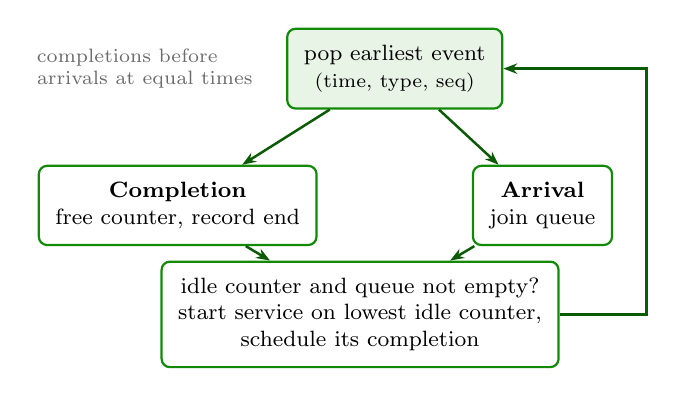
\begin{tikzpicture}[font=\footnotesize, node distance=6mm]
  \node[gbox] (pop) {pop earliest event\\\scriptsize(time, type, seq)};
  \node[box, below left=7mm and -4mm of pop] (cmp) {\textbf{Completion}\\free counter, record end};
  \node[box, below right=7mm and -4mm of pop] (arv) {\textbf{Arrival}\\join queue};
  \node[box, below=7mm of $(cmp)!.5!(arv)$] (start) {idle counter and queue not empty?\\start service on lowest idle counter,\\schedule its completion};
  \draw[arr] (pop) -- (cmp); \draw[arr] (pop) -- (arv);
  \draw[arr] (cmp) -- (start); \draw[arr] (arv) -- (start);
  \draw[arr] (start.east) -- ++(1.1,0) |- (pop.east);
  \node[font=\scriptsize, color=mute, align=left, left=3mm of pop] {completions before\\arrivals at equal times};
\end{tikzpicture}}

% Engine and UI layers.
\newcommand{\archdiagram}{%
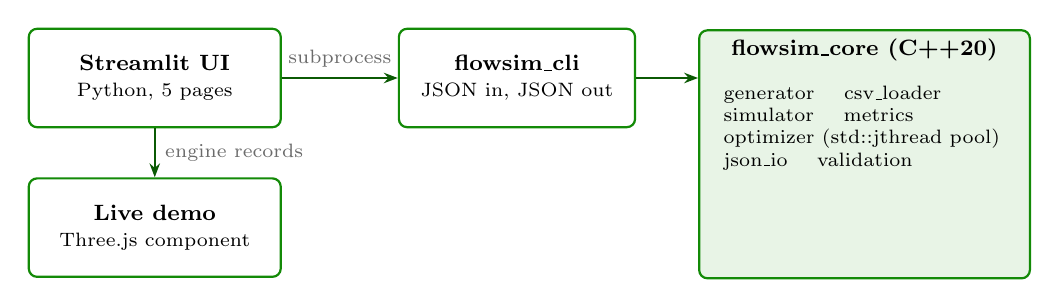
\begin{tikzpicture}[font=\footnotesize]
  \node[box, minimum width=3.2cm, minimum height=1.25cm] (ui) at (0,0) {\textbf{Streamlit UI}\\\scriptsize Python, 5 pages};
  \node[box, minimum width=3.2cm, minimum height=1.25cm] (live) at (0,-1.9) {\textbf{Live demo}\\\scriptsize Three.js component};
  \node[box, minimum width=3.0cm, minimum height=1.25cm] (cli) at (4.6,0) {\textbf{flowsim\_cli}\\\scriptsize JSON in, JSON out};
  \node[gbox, minimum width=4.2cm, minimum height=3.15cm, anchor=north west] (core) at (6.9,.62) {};
  \node[anchor=north, font=\footnotesize\bfseries] at (core.north) {flowsim\_core (C++20)};
  \node[font=\scriptsize, align=left, anchor=north west] at ([shift={(2mm,-6mm)}]core.north west)
    {generator \quad csv\_loader\\simulator \quad metrics\\optimizer (std::jthread pool)\\json\_io \quad validation};
  \draw[arr] (ui.east) -- node[above, font=\scriptsize, color=mute] {subprocess} (cli.west);
  \draw[arr] (cli.east) -- (cli.east -| core.west);
  \draw[arr] (ui) -- node[right, font=\scriptsize, color=mute] {engine records} (live);
\end{tikzpicture}}

% Stacked cost per staffing level.
\newcommand{\costchart}[2]{%
\begin{tikzpicture}
\begin{axis}[fs axis, width=#1, height=#2, ybar stacked, bar width=14pt, ymin=0, ymax=16500,
    xlabel={counters $c$}, ylabel={mean cost per run (INR)}, xtick={3,...,8}, xmin=2.4, xmax=8.6,
    restrict x to domain=3:8, scaled y ticks=false, yticklabel={\pgfmathprintnumber[1000 sep={,}]{\tick}},
    legend columns=3, legend style={at={(0.5,1.02)}, anchor=south}, area legend]
  \addplot[fill=ovgreen, draw=none] table[x=c, y=staffing, col sep=comma] {data/per_counter.csv};
  \addplot[fill=wait, draw=none] table[x=c, y=waiting, col sep=comma] {data/per_counter.csv};
  \addplot[fill=late, draw=none] table[x=c, y=sla, col sep=comma] {data/per_counter.csv};
  \legend{staffing, waiting, SLA penalty}
\end{axis}
\begin{axis}[width=#1, height=#2, ymin=0, ymax=16500, xmin=2.4, xmax=8.6, hide axis]
  \addplot[only marks, mark=*, mark size=1.6pt, ink] table[x=c, y=total, col sep=comma, restrict x to domain=3:8] {data/per_counter.csv};
  \node[font=\scriptsize\bfseries, color=ovdark] at (axis cs:6,8300) {best};
  \node[font=\scriptsize, color=today] at (axis cs:4,11800) {today};
\end{axis}
\end{tikzpicture}}

% People waiting over time in the representative run.
\newcommand{\queuechart}[2]{%
\begin{tikzpicture}
\begin{axis}[fs axis, width=#1, height=#2, xmin=0, xmax=295, ymin=0, xlabel={minutes since 06:00},
    ylabel={people in line}, xtick={0,60,...,300}, legend style={at={(0.02,0.98)}, anchor=north west}]
  \addplot[const plot, today, line width=1pt] table[x=t, y=q, col sep=comma] {data/queue_today.csv};
  \addplot[const plot, ovgreen, line width=1pt] table[x=t, y=q, col sep=comma] {data/queue_plan.csv};
  \legend{{today, 4 lanes},{FlowSim, 6 lanes}}
\end{axis}
\end{tikzpicture}}

% Best counter count against arrival rate.
\newcommand{\sensitivitychart}[2]{%
\begin{tikzpicture}
\begin{axis}[fs axis, width=#1, height=#2, xlabel={arrivals per hour $\lambda$}, ylabel={best counters $c^\ast$},
    ymin=0, ymax=8, xtick={20,28,...,64}, ytick={0,...,8}, axis y line*=left]
  \addplot[const plot mark mid, ovgreen, line width=1.1pt, mark=*, mark size=1.5pt] table[x=rate, y=best, col sep=comma] {data/sensitivity.csv};
  \addplot[dashed, mute, domain=20:64] {x/60*5.5};
  \node[font=\scriptsize, color=mute, rotate=24] at (axis cs:56,4.4) {offered load $\lambda/\mu$};
\end{axis}
\end{tikzpicture}}

\usepackage[colorlinks=true,linkcolor=ovdark,urlcolor=ovdark,citecolor=ovdark]{hyperref}

\titleformat{\section}{\Large\bfseries\color{ovgreen}}{\thesection}{.6em}{}
\titleformat{\subsection}{\large\bfseries\color{ovdark}}{\thesubsection}{.6em}{}
\pagestyle{fancy}\fancyhf{}
\fancyhead[L]{\small\color{mute}FlowSim}\fancyhead[R]{\small\color{mute}MSL304 Course Project}
\fancyfoot[C]{\small\thepage}
\renewcommand{\headrulewidth}{.4pt}
\setlist{itemsep=2pt,topsep=4pt}
\captionsetup{font=small,labelfont={bf,color=ovdark}}
\lstset{basicstyle=\ttfamily\small,backgroundcolor=\color{ovlight},frame=single,rulecolor=\color{ovgreen!40},
  framesep=4pt,columns=fullflexible,keepspaces=true,breaklines=true,showstringspaces=false,
  literate={~}{{\textasciitilde}}1}
\newcommand{\code}[1]{\texttt{#1}}
\newcolumntype{L}{>{\raggedright\arraybackslash}X}

\begin{document}
\begin{titlepage}
  \centering\vspace*{3cm}
  {\color{ovgreen}\rule{\textwidth}{1pt}}\par\vskip14pt
  {\Huge\bfseries\color{ovgreen}FlowSim}\par\vskip8pt
  {\Large Simulation-based staffing for service counters}\par\vskip14pt
  {\color{ovgreen}\rule{\textwidth}{1pt}}\par\vskip2cm
  {\large Sarthak Panda \quad 2022CS51217}\par\vskip6pt
  {\large MSL304 Course Project}\par\vskip6pt
  \href{https://github.com/sarthak-panda/MSL304-Project}{github.com/sarthak-panda/MSL304-Project}\par\vfill
  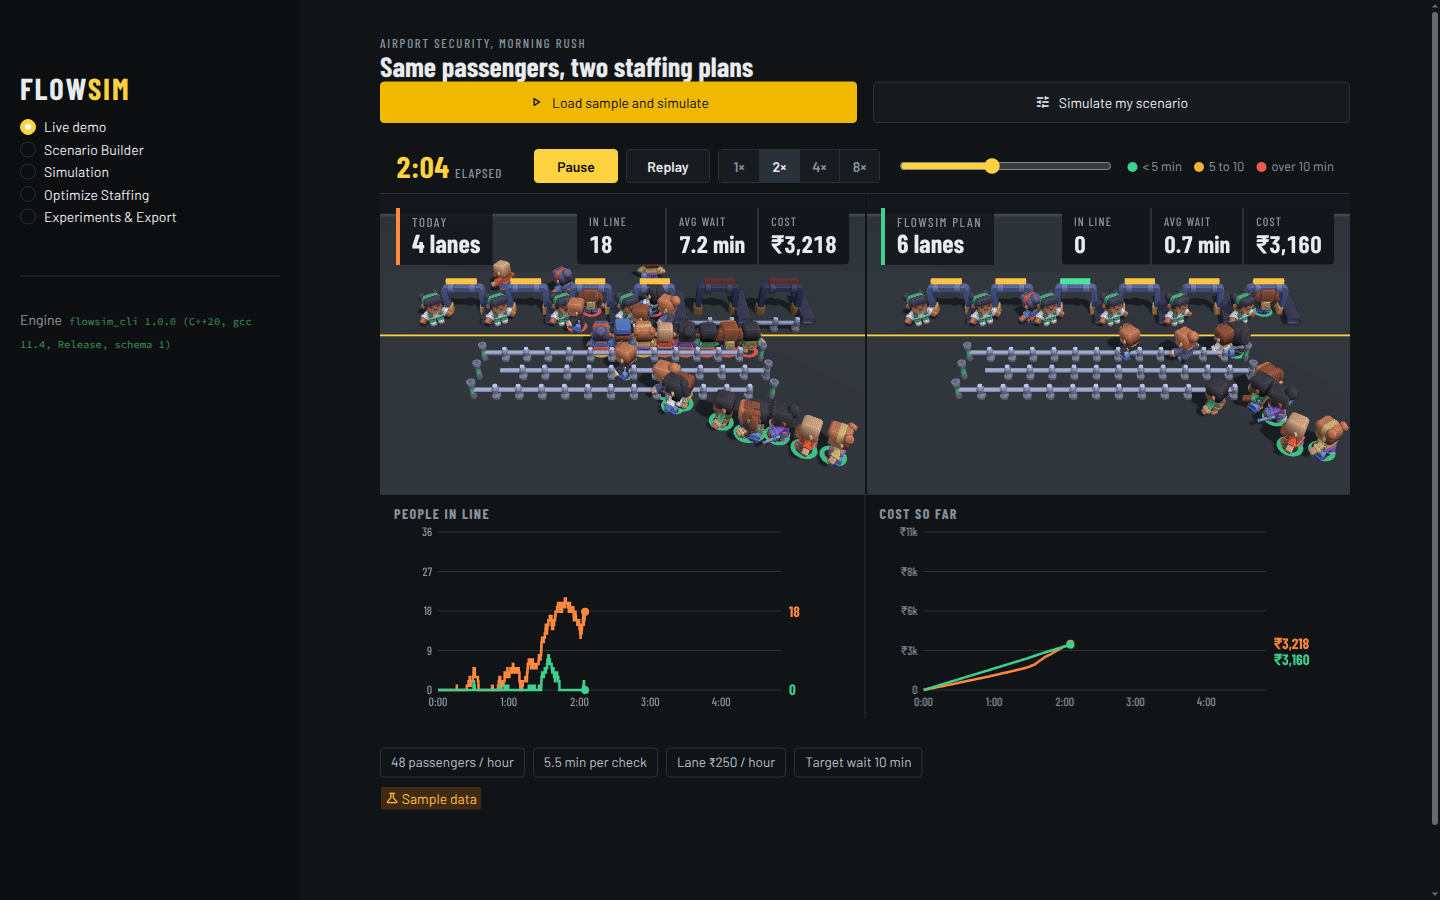
\includegraphics[width=.85\textwidth]{figures/live_demo.png}\par\vskip1cm
\end{titlepage}

\begin{abstract}
FlowSim decides how many identical service counters to open for a queue of arriving customers. It simulates every
customer with a deterministic discrete-event engine written in C++20, prices staff time, customer waiting and late
service in one objective, and evaluates every candidate counter count with common random numbers so the comparison is
fair. A Python and Streamlit interface lets a user build a scenario from synthetic or uploaded data, run a single plan,
run the optimizer, and watch a live 3D replay of today's plan next to the recommended plan. On the sample airport
security scenario (48 passengers per hour, 5.5 minute mean service, 4 counters today) FlowSim recommends 6 counters,
which lowers the mean total cost by 34.0\% and the mean wait from 19.95 to 1.22 minutes. The engine agrees with the
Erlang C formula within 2\% on long stationary runs.
\end{abstract}

\tableofcontents
\newpage

%=====================================================================
\section{Problem and motivation}
Many services put customers in one line in front of several identical counters: airport security lanes, check-in
desks, bank tellers, hospital registration, government offices. The manager chooses how many counters to staff.
\begin{itemize}
  \item With \textbf{too few} counters, the arrival rate exceeds the service capacity. The line grows for as long as the
    rush lasts, waits reach tens of minutes, and customers miss flights or appointments.
  \item With \textbf{too many} counters, waits are near zero but staff are idle much of the time and labour cost rises
    linearly with the counter count.
\end{itemize}
The decision is hard to make by intuition because arrivals are random and bunch up, and because the relation between
capacity and waiting is strongly non-linear near full utilization. A small change in staffing can move the average wait
from twenty minutes to one. Managers therefore tend either to guess or to staff for the worst case.

FlowSim turns the decision into an explicit optimization: put a price on staff time, on customer waiting time and on
every customer served later than a target, simulate the queue for each candidate counter count, and recommend the count
with the lowest expected total cost. The same tool explains the result visually so that a non-specialist can see why the
recommendation is better.

\begin{figure}[H]
\centering
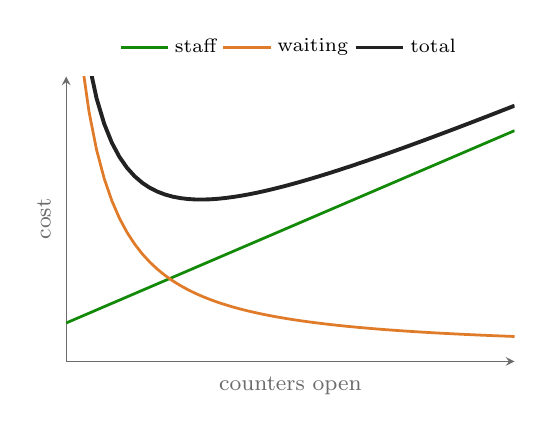
\begin{tikzpicture}
\begin{axis}[fs axis, width=.6\textwidth, height=5.2cm, xlabel={counters open}, ylabel={cost}, domain=1:10, samples=60,
  ymin=0, ymax=10, xtick=\empty, ytick=\empty, legend columns=3, legend style={at={(0.5,1.03)}, anchor=south}]
  \addplot[ovgreen, line width=1pt] {0.75*x+0.6};
  \addplot[today, line width=1pt] {9/(x-0.4)^1.3+0.4};
  \addplot[ink, line width=1.4pt] {0.75*x+0.6+9/(x-0.4)^1.3+0.4};
  \legend{staff, waiting, total}
\end{axis}
\end{tikzpicture}
\caption{The trade-off FlowSim resolves (schematic). Staff cost grows with every counter, waiting cost falls, and the
total has a minimum.}
\end{figure}

\subsection{Scope of the project}
The project proposal described a tool to \emph{configure} a scenario, \emph{simulate} it and \emph{compare} staffing
plans. The implementation delivers:
\begin{enumerate}
  \item a C++20 simulation core and command line tool \code{flowsim\_cli};
  \item an exhaustive staffing optimizer with replications, common random numbers and multi-threading;
  \item a Streamlit user interface with five pages, including a Three.js live replay;
  \item unit, integration, sanitizer and UI tests, run in GitHub Actions;
  \item a static replay site that can be published with GitHub Pages.
\end{enumerate}

%=====================================================================
\section{Terms and notation}
\begin{table}[H]
\centering\small
\begin{tabularx}{\textwidth}{@{}l L@{}}
\toprule
Term & Meaning \\
\midrule
Customer / passenger & One person who joins the line, waits, is served and leaves. Indexed by $i=1,\dots,n$. \\
Counter / lane & One server. All counters are identical and serve one customer at a time. \\
Shared FIFO queue & A single line in front of all counters; the customer who arrived first is served first. \\
Arrival window & The period during which customers arrive, $[0, H]$ minutes. \\
Arrival rate $\lambda$ & Expected arrivals per unit time (input in passengers per hour). \\
Service time $S_i$ & Time a counter spends on customer $i$; mean $1/\mu$. \\
Offered load $a$ & $a=\lambda/\mu$, the average number of busy counters needed to keep up. \\
Utilization $\rho$ & $\rho = a/c$ in theory; in the engine, busy counter-minutes divided by $c\cdot T$. \\
Arrival time $A_i$ & Time customer $i$ joins the line. \\
Start time $B_i$ & Time a counter starts serving customer $i$. \\
Departure $D_i$ & $D_i=B_i+S_i$, time service ends. \\
Wait $W_i$ & $W_i = B_i - A_i \ge 0$, time spent in line, excluding service. \\
Finish time $T$ & $T=\max_i D_i$, completion of the last service (the drain time). \\
SLA target $S$ & A wait threshold in minutes. A customer is \emph{late} if $W_i > S$ (strict). \\
Service level & Percentage of customers with $W_i \le S$, called ``on time'' in the UI. \\
$p95$ wait & 95th percentile of the waits in one run. \\
Replication & One independent simulated day with its own random arrivals and service times. \\
Seed & Integer that fixes the random number stream, so a run can be reproduced exactly. \\
Common random numbers (CRN) & Using the same simulated customers for every candidate counter count. \\
Baseline & The current staffing $c_0$ (``today'') used for comparison. \\
\bottomrule
\end{tabularx}
\caption{Terms used in this report.}
\end{table}

%=====================================================================
\section{Mathematical model}
\subsection{Queueing system}
FlowSim models a multi-server queue with one unlimited shared FIFO line feeding $c$ identical parallel counters
(Figure~\ref{fig:queue}). In Kendall notation the synthetic model is $M/M/c$ (exponential service) or $M/D/c$ (fixed
service) over a finite arrival window, with all customers served after the window closes.

\begin{figure}[H]\centering\queuediagram\caption{One shared FIFO queue feeding $c$ identical counters.}\label{fig:queue}\end{figure}

Assumptions:
\begin{itemize}
  \item Counters are identical, open for the whole run, and never take breaks.
  \item The queue has unlimited capacity. Customers never balk (refuse to join), renege (leave the line) or jockey.
  \item Discipline is first come, first served. A free counter takes the customer at the head of the line.
  \item When several counters are idle, the lowest-numbered idle counter is used. This only affects which counter is
    shown, not any metric.
  \item After the arrival window closes, counters stay open until the line is empty, so all $n$ customers are served.
\end{itemize}

\subsection{Synthetic arrivals and service times}
Arrivals follow a homogeneous Poisson process with rate $\lambda$ per minute ($\lambda = \lambda_{\text{hour}}/60$).
Equivalently, inter-arrival times are independent exponential random variables:
\[
  A_1 = X_1,\qquad A_{i+1} = A_i + X_{i+1},\qquad X_k \stackrel{\text{iid}}{\sim} \operatorname{Exp}(\lambda),\qquad
  \Pr(X_k > x)=e^{-\lambda x}.
\]
Generation stops at the first arrival after the window $H$, so the number of customers $n$ is Poisson with mean
$\lambda H$. Service times are independent of arrivals and of each other:
\[
  S_i \sim \operatorname{Exp}(\mu)\ \text{with}\ \mathbb{E}[S_i]=1/\mu \qquad\text{or}\qquad S_i = 1/\mu\ \text{(fixed)}.
\]
Each replication $r$ uses the pseudo-random generator \code{std::mt19937\_64} seeded with $s+r$, where $s$ is the scenario
seed. The same seed always produces the same customers on every platform that uses the same standard library.

\subsection{CSV mode}
Instead of generating customers, the user can upload a CSV with the columns
\code{passenger\_id}, \code{arrival\_time\_min} and \code{service\_time\_min}. Each row is validated (non-negative finite numbers, unique
identifiers, no missing fields). Because the data is fixed there is no randomness, so the optimizer runs one replication
per counter count, and synthetic-only parameters (rate, mean service, distribution, seed) are rejected.

\subsection{Sample path and the event recursion}
For a FIFO queue with $c$ servers, start times satisfy
\[
  B_i = \max\bigl(A_i,\ F_i\bigr),
\]
where $F_i$ is the time the earliest counter becomes free once customers $1,\dots,i-1$ have started. For $c=1$ this reduces to the Lindley recursion $W_{i+1}=\max(0, W_i + S_i - X_{i+1})$. FlowSim does not use the
closed recursion directly. It runs an event simulation (Section~\ref{sec:des}) that produces the same values and also
records the queue length over time and which counter served each customer.

\subsection{Metrics of one run}
For one run with counter count $c$:
\begin{align*}
  \bar W &= \frac1n\sum_{i=1}^n W_i \quad\text{(mean wait)}, &
  W_{\max} &= \max_i W_i, \\
  W_{95} &= \text{95th percentile of } \{W_i\}, &
  \text{SL} &= \frac{100}{n}\,\#\{i: W_i \le S\} \quad\text{(service level, \%)}, \\
  U &= \frac{100}{c\,T}\sum_{i=1}^n S_i \quad\text{(utilization, \%)}, &
  Q_{\max} &= \max_t Q(t) \quad\text{(longest line)},
\end{align*}
where $Q(t)$ is the number waiting (not in service) at time $t$. Percentiles use the nearest-rank method on the sorted waits. The engine also reports the mean time in system $\frac1n\sum_i (D_i-A_i)$ and the finish time $T$.

\subsection{Objective function}
Let $r_s$ be the cost of one counter per hour, $r_w$ the cost of one passenger-hour of waiting and $p$ the penalty per late
passenger. For one run with $c$ counters the cost is
\[
  J(c) \;=\; \underbrace{\frac{c\, r_s\, T}{60}}_{\text{staffing}}
   \;+\; \underbrace{\frac{r_w}{60}\sum_{i=1}^{n} W_i}_{\text{waiting}}
   \;+\; \underbrace{p\cdot \#\{i : W_i > S\}}_{\text{SLA penalty}} .
\]
Times are in minutes, hence the divisions by 60. Staffing is charged until the last service ends ($T$), not only for the
arrival window, because the counters must remain open to clear the line. FlowSim chooses
\[
  c^\star \;=\; \arg\min_{c_{\min}\le c\le c_{\max}} \ \mathbb{E}\bigl[J(c)\bigr],
  \qquad
  \widehat{\mathbb{E}}[J(c)] = \frac1R\sum_{r=0}^{R-1} J_r(c),
\]
where $J_r(c)$ is the cost of replication $r$. The engine also reports the sample standard deviation of $J_r(c)$ and the
mean of every component, so a user can see whether a recommendation is driven by staff cost, waiting or penalties.

\paragraph{Why a minimum exists.} Staffing is roughly linear in $c$. As $c$ approaches the offered load $a$ from above, the
waiting term grows like $1/(c-a)$ (see Equation~\eqref{eq:erlang}), and for $c\le a$ the line grows without bound during
the rush. The sum is therefore large for small $c$, grows linearly for large $c$, and has a minimum in between.

\paragraph{Tie rule.} If two counter counts have a mean cost within a relative tolerance of $10^{-9}$, the smaller count
wins, because it uses fewer staff for the same cost.

\paragraph{Relation to the proposal.} The proposal suggested a weighted objective of staffing, average wait and the
95th percentile wait. The implemented objective keeps the same intent but uses monetary weights, which are easier for a
manager to set, and replaces the percentile term by an explicit penalty per late passenger. The $p95$ wait is still
reported for every plan.

\subsection{Queueing theory reference: Erlang C}
For a stationary $M/M/c$ queue with $a=\lambda/\mu<c$, the probability that an arriving customer waits and the mean
wait in queue are
\begin{equation}
  P_W = \frac{\dfrac{a^c}{c!}\dfrac{1}{1-\rho}}{\displaystyle\sum_{k=0}^{c-1}\frac{a^k}{k!} + \frac{a^c}{c!}\frac{1}{1-\rho}},
  \qquad
  W_q = \frac{P_W}{c\mu-\lambda} = \frac{P_W}{\mu\,(c-a)},\qquad \rho=\frac ac.
  \label{eq:erlang}
\end{equation}
The finite morning window is not stationary, so FlowSim does not use this formula to decide. It uses it to validate the
engine on long runs (Section~\ref{sec:validation}).

%=====================================================================
\section{Simulation and optimization algorithms}
\subsection{Discrete-event simulation}\label{sec:des}
The simulator jumps from event to event instead of stepping a clock. There are two event types: \emph{arrival} of a
customer and \emph{completion} of a service.

\begin{figure}[H]\centering\eventdiagram\caption{The event loop of the simulator.}\end{figure}

\begin{algorithm}[H]
\caption{Simulate one run with $c$ counters}
\begin{algorithmic}[1]
\State push an arrival event for every customer; mark all counters idle (min-heap by counter number)
\While{the event heap is not empty}
  \State pop the earliest event $e$ (order: time, then completion before arrival, then sequence number)
  \If{$e$ is a completion on counter $k$} \State record $D_i$; mark $k$ idle
  \Else \State append the customer to the FIFO queue
  \EndIf
  \While{an idle counter exists \textbf{and} the queue is not empty}
    \State take the lowest idle counter $k$ and the queue head $i$; set $B_i\gets t$, $W_i\gets t-A_i$
    \State push a completion event for counter $k$ at $t+S_i$
  \EndWhile
  \State record $(t, Q(t))$ in the queue trace if it changed
  \If{the number of processed events exceeds the safety cap} \State stop with \code{INCOMPLETE\_SIMULATION} \EndIf
\EndWhile
\end{algorithmic}
\end{algorithm}

\paragraph{Determinism.} The order of simultaneous events is fixed: a completion at time $t$ is processed before an
arrival at time $t$, so a counter that frees up at the exact moment a customer arrives can serve that customer with zero
wait. Ties among equal arrivals are broken by input order. Given the same input, the engine always produces the same
output, which makes testing and CRN possible.

\paragraph{Complexity.} Each customer generates two events and each heap operation costs $O(\log n)$ or $O(\log c)$,
so one run costs $O(n\log n)$ time and $O(n)$ memory.

\subsection{Exhaustive search with common random numbers}
The decision variable is a small integer, so FlowSim evaluates every $c\in[c_{\min},c_{\max}]$. For each replication
$r$ it generates the customers once and reuses them for every $c$ (common random numbers). Then
\[
  \operatorname{Var}\bigl[J_r(c_1)-J_r(c_2)\bigr]
  = \operatorname{Var}[J_r(c_1)] + \operatorname{Var}[J_r(c_2)] - 2\operatorname{Cov}[J_r(c_1),J_r(c_2)],
\]
and the covariance is strongly positive because a busy day is busy for every plan. Differences between plans are
therefore much less noisy than with independent samples, and the ranking of plans is stable with only a few
replications.

\subsection{Parallel execution}
The $(c,r)$ pairs are independent tasks. They are executed on a pool of \code{std::jthread} workers that take task
indices from an atomic counter. Each task writes its result into its own pre-allocated slot, so no locks are needed, and
results are aggregated in a fixed order afterwards. Parallel output is therefore identical to sequential output, which
is checked by a unit test. An exception in a worker is captured and re-thrown on the main thread.

%=====================================================================
\section{Implementation}
\subsection{Architecture}
\begin{figure}[H]\centering\archdiagram\caption{Components and how they talk to each other.}\end{figure}

The C++ engine is the single source of truth. Python never simulates; it builds a scenario document, calls the engine
as a subprocess with an argument list (no shell), and displays the JSON it returns.

\begin{table}[H]\centering\small
\begin{tabularx}{\textwidth}{@{}l L@{}}
\toprule
File & Role \\
\midrule
\code{include/flowsim/types.hpp} & Scenario, passenger, run result and optimizer result types \\
\code{src/passenger\_generator.cpp} & Seeded Poisson arrivals and service times \\
\code{src/csv\_loader.cpp} & Strict parsing of passenger CSV files \\
\code{src/simulator.cpp} & Event loop, FIFO queue, counter assignment, queue trace \\
\code{src/metrics.cpp} & Waits, percentiles, service level, utilization, cost components \\
\code{src/optimizer.cpp} & Exhaustive search, CRN, thread pool, tie rule, baseline \\
\code{src/validation.cpp} & Field-level validation with error codes \\
\code{src/json\_io.cpp}, \code{src/main.cpp} & Versioned JSON schema and the \code{flowsim\_cli} commands \\
\code{ui/flowsim\_client.py} & Finds and runs the engine, maps errors to \code{FlowSimError} \\
\code{ui/scenario.py} & Sample scenario, scenario documents, CSV checks \\
\code{ui/app.py}, \code{ui/charts.py} & Streamlit pages and Plotly charts \\
\code{ui/live\_demo/} & Streamlit component with the Three.js replay \\
\code{bench/benchmark.cpp} & Sequential versus parallel benchmark \\
\bottomrule
\end{tabularx}
\caption{Main source files.}
\end{table}

\subsection{Command line contract}
\code{flowsim\_cli} has three commands: \code{version}, \code{simulate} (one counter count) and \code{optimize}. Input and
output are JSON documents with \code{"schema\_version": 1}. Errors are reported with a code, a message and the offending
field, for example \code{scenario.arrival\_rate\_per\_hour}.
\begin{table}[H]\centering\small
\begin{tabular}{@{}cl@{}}\toprule Exit code & Meaning\\\midrule
0 & success\\ 1 & internal error\\ 2 & usage error (bad arguments)\\ 3 & invalid input\\ 4 & incomplete simulation (safety cap)\\
\bottomrule\end{tabular}\caption{Exit codes of \code{flowsim\_cli}.}\end{table}

\subsection{Python user interface}
The Streamlit app has five pages:
\begin{description}[style=nextline,leftmargin=1em]
  \item[Live demo] Landing page with a short explanation and the objective. \emph{Load sample and simulate} runs the
    optimizer and starts the side-by-side replay; \emph{Simulate my scenario} does the same with the user's scenario.
  \item[Scenario Builder] Synthetic parameters or a CSV upload, costs, SLA, candidate range, replications and seed, with
    validation messages next to each field.
  \item[Simulation] One plan in detail: KPIs, a timeline bar per customer, queue length and utilization over time.
  \item[Optimize Staffing] All candidate counts, the stacked cost chart, the recommendation and a short reason.
  \item[Experiments \& Export] Re-run with a new seed, a history of runs, and downloads as CSV and JSON.
\end{description}

\subsection{Live 3D replay}
The live demo is a custom Streamlit component written with Three.js. It shows two security halls: \emph{Today} with the
current counters and \emph{FlowSim plan} with the recommended counters. Both use the same passengers of the same
replication. Each passenger appears at its engine arrival time $A_i$, walks to the line, starts service at $B_i$ at the
counter chosen by the engine and leaves at $D_i$. Only the walking between these points is animation. Above each hall,
boards show the people in line, the average wait so far and the cost so far; below, two charts draw the queue length
and cumulative cost as the clock runs. A ring under each passenger is coloured by wait relative to the target. Controls
offer play, pause, replay, speeds up to $8\times$ and a timeline slider. The 3D models (CC0), Three.js and fonts are
stored in the repository, so the demo works offline.

\begin{figure}[H]
\centering
\begin{subfigure}{.49\textwidth}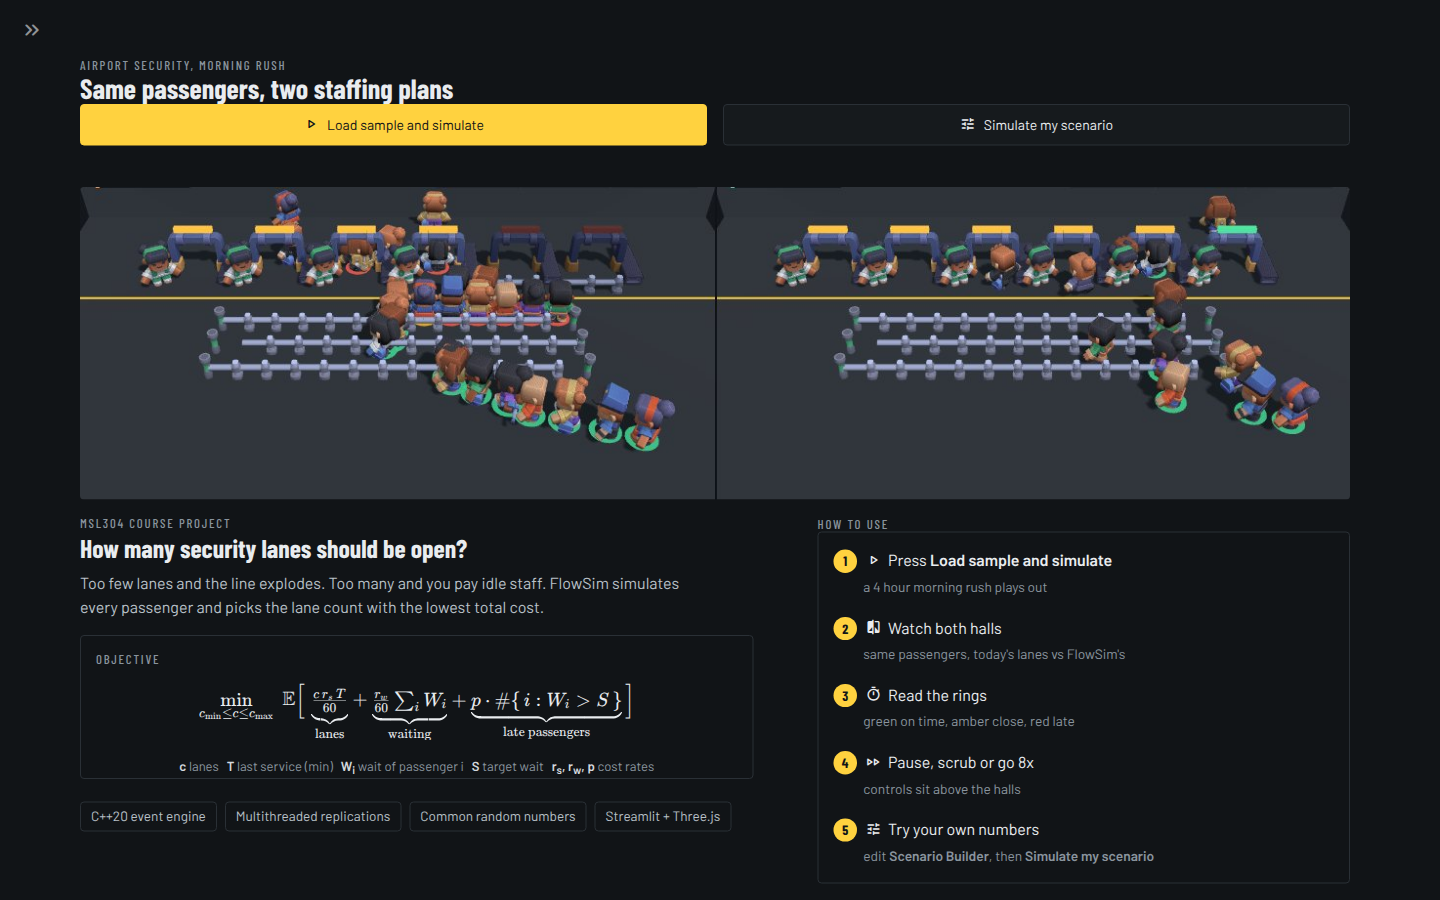
\includegraphics[width=\linewidth]{figures/landing.png}\caption{Landing page}\end{subfigure}\hfill
\begin{subfigure}{.49\textwidth}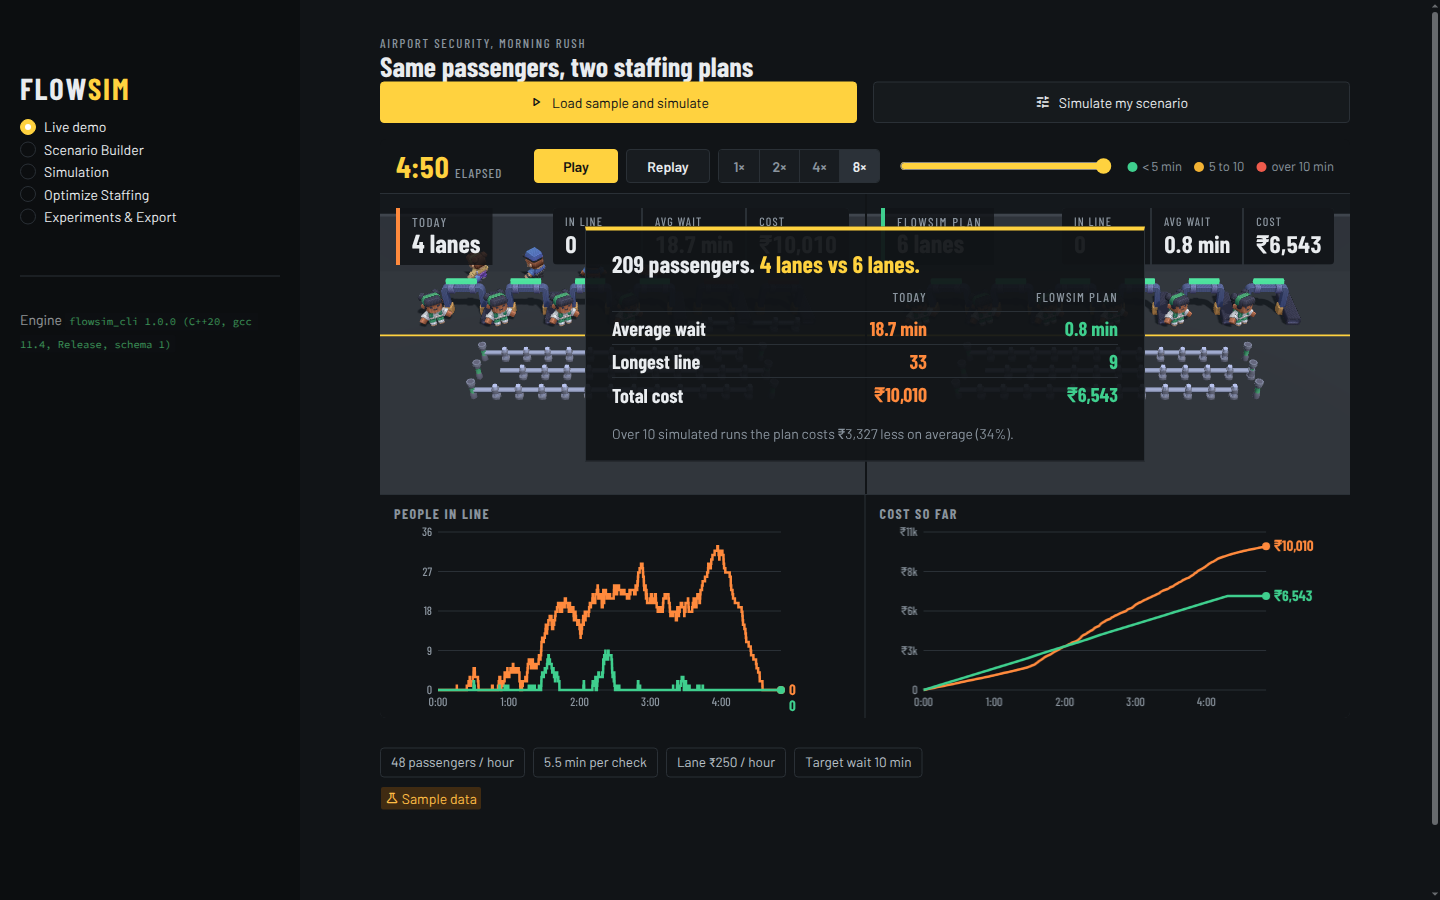
\includegraphics[width=\linewidth]{figures/live_demo_result.png}\caption{Replay result}\end{subfigure}
\caption{Live demo page before and after a replay.}
\end{figure}

\begin{figure}[H]
\centering
\begin{subfigure}{.49\textwidth}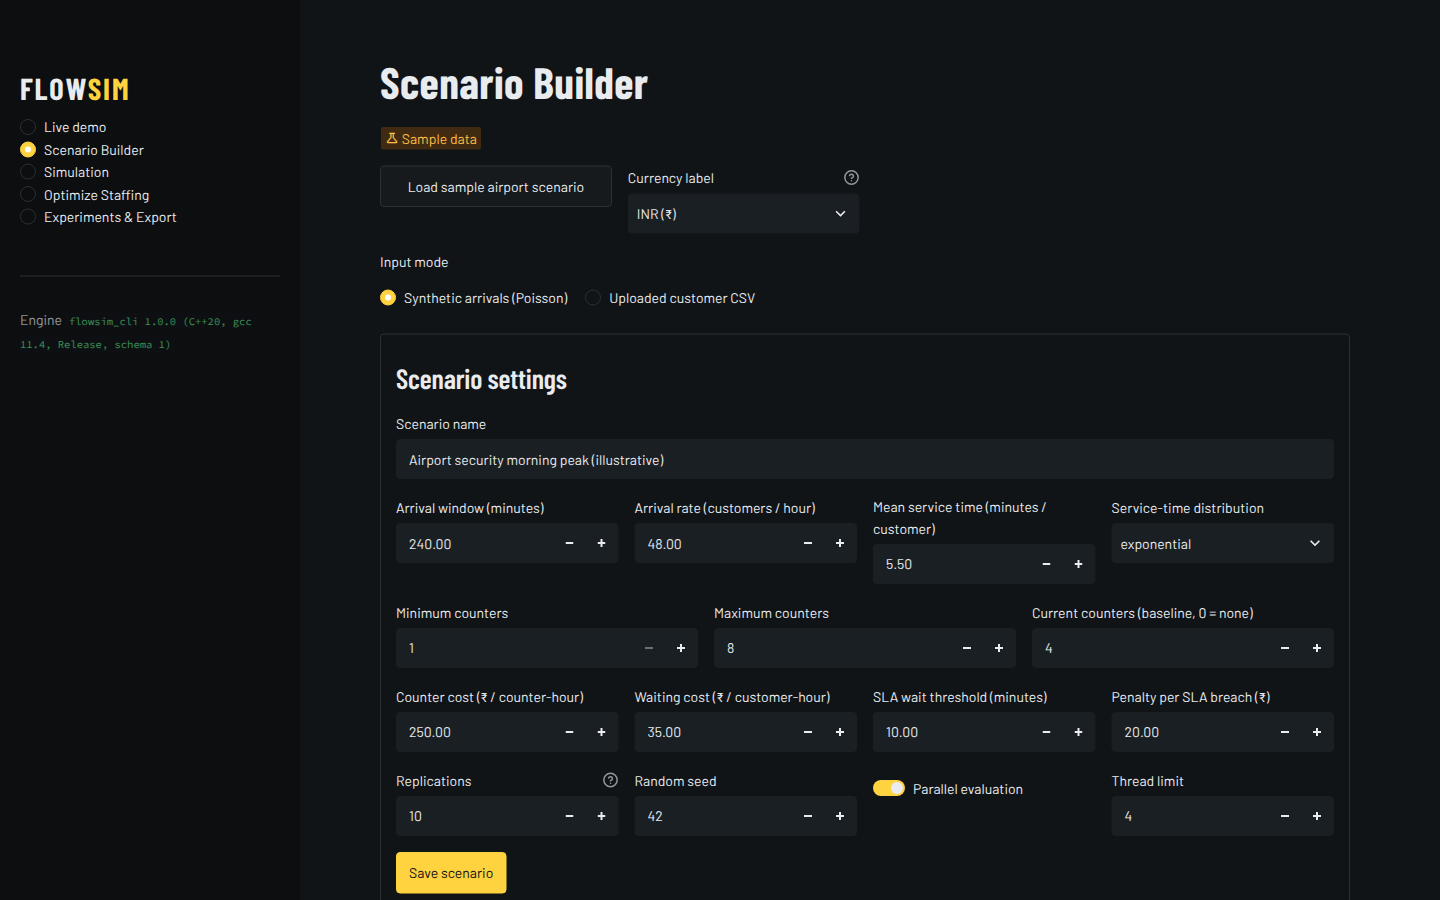
\includegraphics[width=\linewidth]{figures/scenario_builder.png}\caption{Scenario Builder}\end{subfigure}\hfill
\begin{subfigure}{.49\textwidth}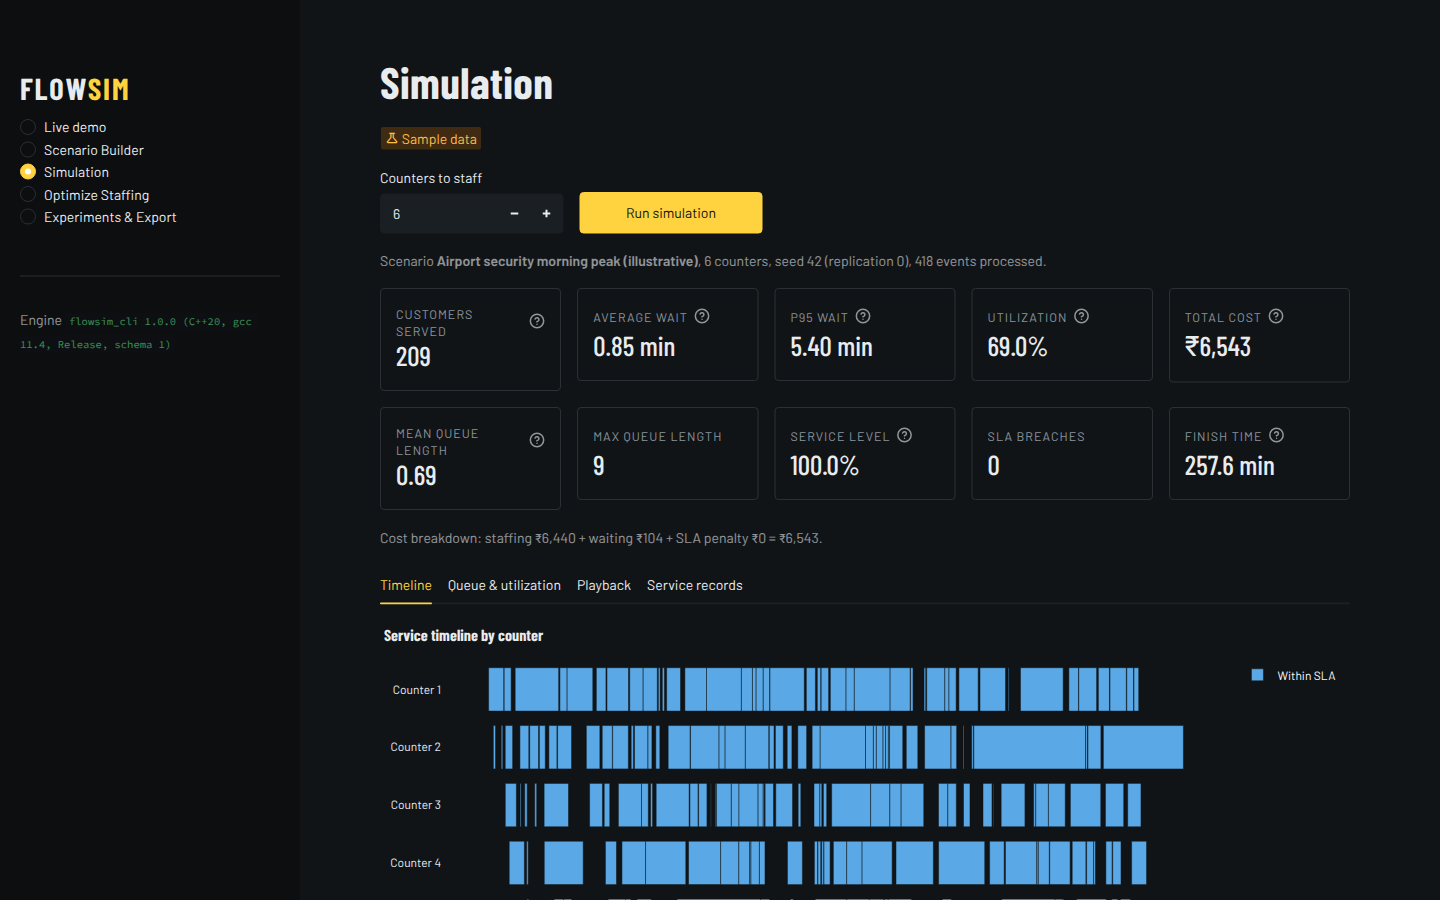
\includegraphics[width=\linewidth]{figures/simulation.png}\caption{Simulation}\end{subfigure}\\[6pt]
\begin{subfigure}{.49\textwidth}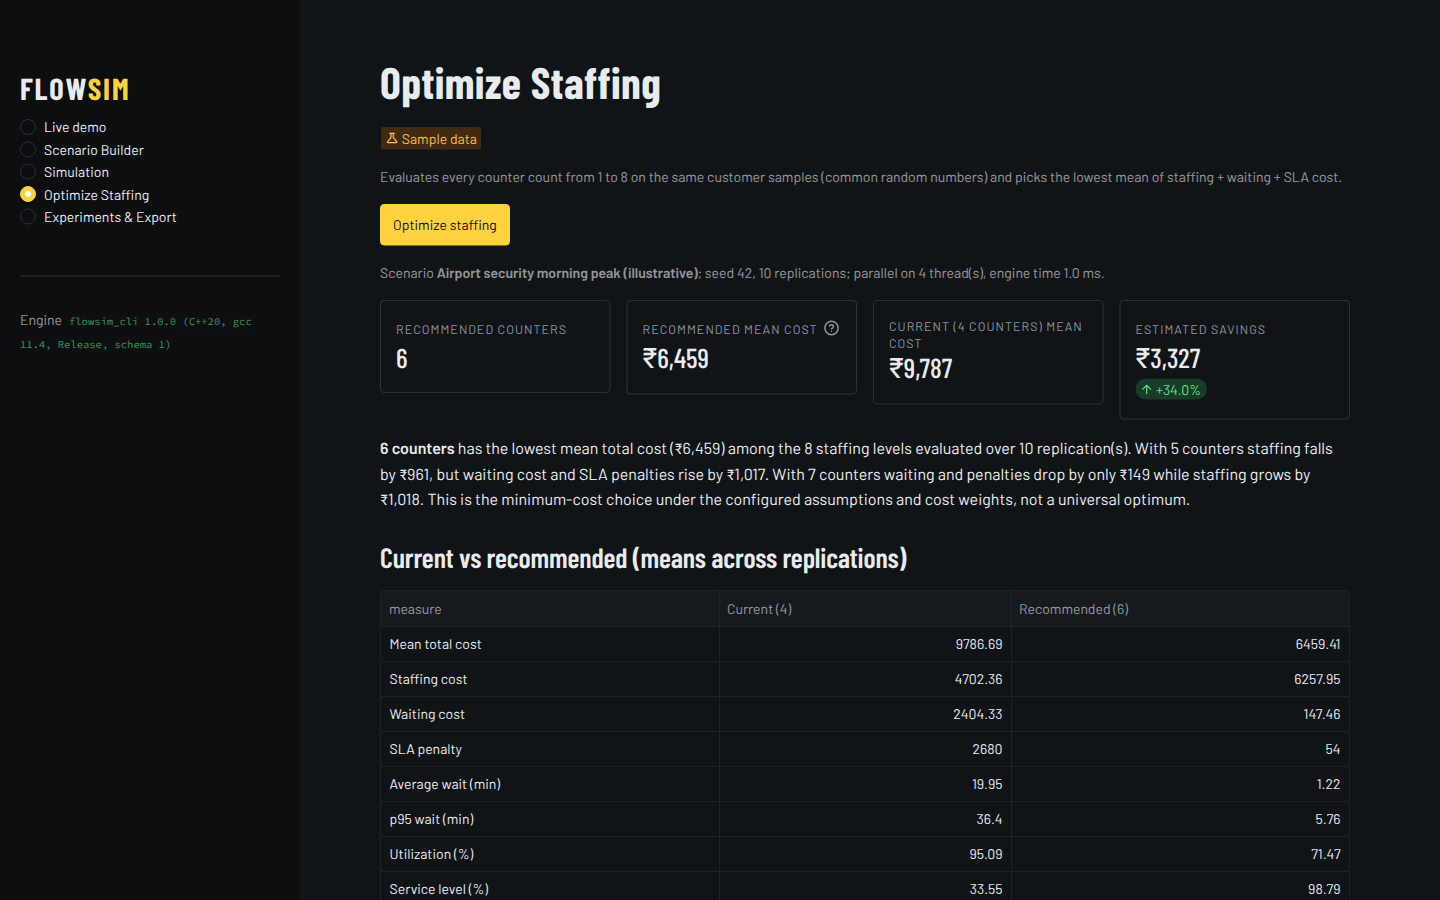
\includegraphics[width=\linewidth]{figures/optimize_staffing.png}\caption{Optimize Staffing}\end{subfigure}\hfill
\begin{subfigure}{.49\textwidth}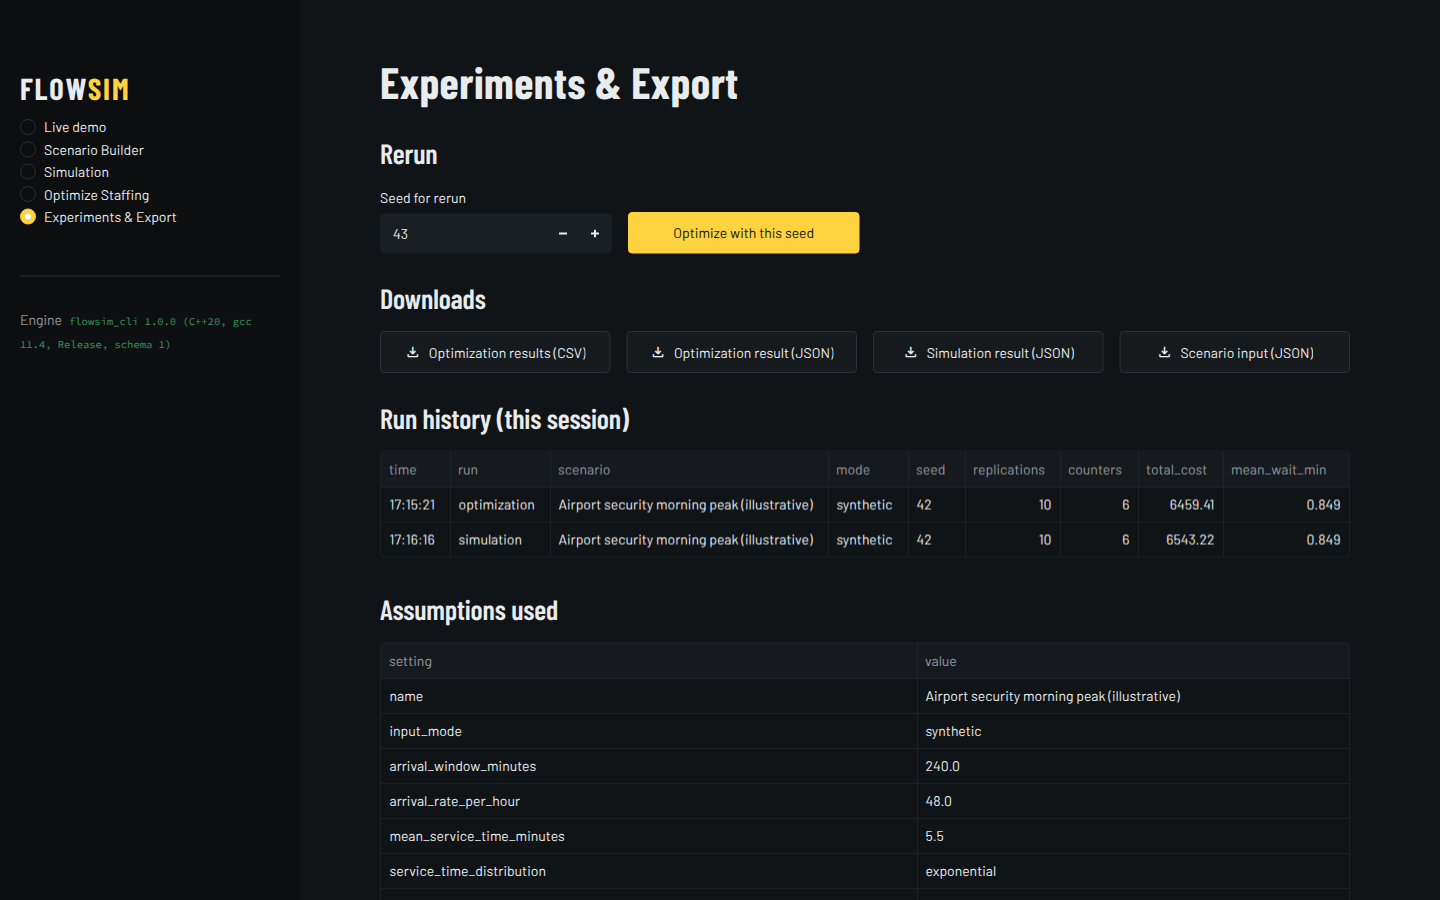
\includegraphics[width=\linewidth]{figures/experiments_export.png}\caption{Experiments \& Export}\end{subfigure}
\caption{The other pages of the platform.}
\end{figure}

\subsection{Testing and continuous integration}
\begin{itemize}
  \item \textbf{C++ unit tests} (33): empty input, single customer, FIFO order, completion before arrival at equal
    times, no counter overlap, conservation of customers, hand-computed metric fixtures, strict SLA, reproducibility,
    invalid input, the safety cap, optimizer range and tie rule, CRN, parallel equals sequential, worker exceptions, CSV
    runs.
  \item \textbf{CLI tests} through CTest check commands, exit codes and JSON errors.
  \item \textbf{Python tests} (35) run the real engine through the client and drive every Streamlit page headlessly.
  \item \textbf{Sanitizers}: AddressSanitizer with UndefinedBehaviorSanitizer, and ThreadSanitizer.
  \item \textbf{GitHub Actions} runs all of the above on every pull request and builds the static replay site.
\end{itemize}

\begin{table}[H]\centering\small
\begin{tabular}{@{}rrrr@{}}\toprule passengers & sequential & 8 threads & speedup\\\midrule
1{,}007 & 3.5 ms & 0.9 ms & 3.9$\times$\\ 9{,}998 & 32.4 ms & 4.7 ms & 6.9$\times$\\ 99{,}838 & 363.6 ms & 43.7 ms & 8.3$\times$\\
\bottomrule\end{tabular}
\caption{Benchmark of 32 runs (4 replications $\times$ 8 counter counts) on an 8 vCPU machine. Results were identical in
both modes.}\end{table}

%=====================================================================
\section{Results on the sample scenario}
\subsection{Scenario}
\begin{table}[H]\centering\small
\begin{tabular}{@{}lr@{\qquad}lr@{}}\toprule
Arrival window $H$ & 240 min & Counter cost $r_s$ & 250 per hour\\
Arrival rate $\lambda$ & 48 per hour & Waiting cost $r_w$ & 35 per passenger-hour\\
Mean service $1/\mu$ & 5.5 min, exponential & SLA target $S$ & 10 min\\
Today $c_0$ & 4 counters & Late penalty $p$ & 20 per passenger\\
Candidates & 1 to 8 & Replications $R$, seed $s$ & 10, 42\\
\bottomrule\end{tabular}
\caption{Sample airport security scenario (\code{config/example\_scenario.json}). Costs are illustrative, in INR.}
\end{table}
The offered load is $a = 48\times5.5/60 = 4.4$ busy counters. With 4 counters, $\rho=1.1>1$: capacity is below demand,
so the line can only grow until arrivals stop. This is visible in the queue chart below.

\subsection{Cost by staffing level}
\begin{figure}[H]\centering\costchart{.8\textwidth}{6.5cm}
\caption{Mean cost components over 10 replications for $c=3,\dots,8$ ($c=1,2$ cost 57{,}836 and 26{,}091 and are left
off the chart).}\end{figure}

\begin{table}[H]\centering\small
\pgfplotstabletypeset[col sep=comma, columns={c,staffing,waiting,sla,total,sd,wait,p95,service_level,util,maxq,finish},
  columns/c/.style={column name=$c$},
  columns/staffing/.style={column name=staff, fixed, precision=0, 1000 sep={,}},
  columns/waiting/.style={column name=waiting, fixed, precision=0, 1000 sep={,}},
  columns/sla/.style={column name=SLA, fixed, precision=0, 1000 sep={,}},
  columns/total/.style={column name=total, fixed, precision=1, 1000 sep={,}},
  columns/sd/.style={column name=sd, fixed, precision=0, 1000 sep={,}},
  columns/wait/.style={column name=$\bar W$, fixed, precision=2},
  columns/p95/.style={column name=$W_{95}$, fixed, precision=1},
  columns/service_level/.style={column name=SL \%, fixed, precision=1},
  columns/util/.style={column name=$U$ \%, fixed, precision=1},
  columns/maxq/.style={column name=$Q_{\max}$, fixed, precision=1},
  columns/finish/.style={column name=$T$, fixed, precision=0},
  every head row/.style={before row=\toprule, after row=\midrule}, every last row/.style={after row=\bottomrule},
  every row no 3/.style={before row=\rowcolor{today!15}}, every row no 5/.style={before row=\rowcolor{ovlight}}]
  {data/per_counter.csv}
\caption{Mean over 10 replications for every candidate. Costs in INR, times in minutes. Orange: today. Green:
recommended.}\label{tab:all}
\end{table}

FlowSim recommends $c^\star=6$. Compared with today's 4 counters, the mean total cost falls from 9{,}786.7 to 6{,}459.4,
a saving of 3{,}327.3 (34.0\%), and the mean wait falls by 93.9\%. The neighbours confirm the minimum: 5 counters save
961 in staff cost but add 1{,}017 in waiting and penalties, and 7 counters add 1{,}018 in staff cost to save only 149.
Utilization at 6 counters is 71.5\%, a comfortable level, while at 4 counters it is 95.1\% and only a third of passengers
are served within 10 minutes. The standard deviation column shows how much the cost varies from day to day; at 4
counters it is almost ten times larger than at 6, so the current plan is not only more expensive but also less
predictable.

\subsection{One replication in detail}
\begin{figure}[H]\centering\queuechart{.75\textwidth}{6cm}
\caption{People in line over time for replication 0, same 209 passengers, 4 versus 6 counters.}\end{figure}

\begin{table}[H]\centering\small
\begin{tabular}{@{}lrr@{}}\toprule replication 0 & today (4) & FlowSim (6)\\\midrule
mean wait (min) & 18.74 & 0.85\\ $p95$ wait (min) & 36.1 & 5.4\\ longest line & 33 & 9\\ service level (\%) & 31.1 & 100.0\\
utilization (\%) & 91.8 & 69.0\\ staffing cost & 4{,}844.6 & 6{,}439.7\\ waiting cost & 2{,}285.2 & 103.5\\
SLA penalty & 2{,}880.0 & 0.0\\ total cost & 10{,}009.8 & 6{,}543.2\\\bottomrule\end{tabular}
\caption{The run shown in the live demo.}\end{table}

\begin{figure}[H]\centering
\begin{tikzpicture}
\begin{axis}[fs axis, width=.75\textwidth, height=5.5cm, ybar, bar width=9pt, xlabel={wait (minutes)}, ylabel={passengers},
  xtick={0,5,...,45}, xticklabels={0--5,5--10,10--15,15--20,20--25,25--30,30--35,35--40,40--45,45+},
  x tick label style={font=\scriptsize}, ymin=0, legend style={at={(0.98,0.98)}, anchor=north east}]
  \addplot[fill=today, draw=none] table[x=lo, y=n, col sep=comma] {data/wait_hist_today.csv};
  \addplot[fill=ovgreen, draw=none] table[x=lo, y=n, col sep=comma] {data/wait_hist_plan.csv};
  \legend{{today, 4 lanes},{FlowSim, 6 lanes}}
\end{axis}
\end{tikzpicture}
\caption{Distribution of waits in replication 0. With 6 counters every passenger waits less than 10 minutes.}
\end{figure}

\subsection{Validation against Erlang C}\label{sec:validation}
To check the engine, it was run on long synthetic scenarios (one week, 10{,}080 minutes, 20 replications) with the
sample arrival and service rates, and the simulated mean wait was compared with Equation~\eqref{eq:erlang}.
\begin{table}[H]\centering\small
\pgfplotstabletypeset[col sep=comma, columns={c,rho,sim,theory,util_sim,err_pct},
  columns/c/.style={column name=$c$}, columns/rho/.style={column name=$\rho$, fixed, precision=2},
  columns/sim/.style={column name=simulated $W_q$ (min), fixed, precision=3},
  columns/theory/.style={column name=Erlang C $W_q$ (min), fixed, precision=3},
  columns/util_sim/.style={column name=simulated $U$ \%, fixed, precision=1},
  columns/err_pct/.style={column name=difference \%, fixed, precision=1},
  every head row/.style={before row=\toprule, after row=\midrule}, every last row/.style={after row=\bottomrule}]
  {data/erlang.csv}
\caption{Simulated versus theoretical mean wait in queue for $M/M/c$. All within 2\%, and the simulated utilization matches
$\rho$.}\end{table}

\subsection{Sensitivity to demand}
\begin{figure}[H]\centering\sensitivitychart{.7\textwidth}{6cm}
\caption{Best counter count as the arrival rate changes from 20 to 64 per hour (other parameters as in the sample,
candidates 1 to 12). The recommendation stays above the offered load $\lambda/\mu$ by a margin of one to two counters.}
\end{figure}

\begin{table}[H]\centering\small
\pgfplotstabletypeset[col sep=comma, columns={rate,load,best,base_cost,best_cost,savings_pct,best_wait},
  columns/rate/.style={column name=$\lambda$ (per hour)}, columns/load/.style={column name=load $a$, fixed, precision=2},
  columns/best/.style={column name=$c^\star$},
  columns/base_cost/.style={column name=cost at 4, fixed, precision=0, 1000 sep={,}},
  columns/best_cost/.style={column name=cost at $c^\star$, fixed, precision=0, 1000 sep={,}},
  columns/savings_pct/.style={column name=saving \%, fixed, precision=1},
  columns/best_wait/.style={column name=$\bar W$ at $c^\star$, fixed, precision=2},
  every head row/.style={before row=\toprule, after row=\midrule}, every last row/.style={after row=\bottomrule}]
  {data/sensitivity.csv}
\caption{Demand sensitivity. A saving of 0 means today's 4 counters are already optimal.}\end{table}

\subsection{CSV mode on the sample passenger file}
\code{data/sample\_passengers.csv} holds 60 synthetic passengers. Running the optimizer on it with candidates 1 to 6 (one
fixed replication each) gives:
\begin{table}[H]\centering\small
\pgfplotstabletypeset[col sep=comma, columns/c/.style={column name=$c$},
  columns/total/.style={column name=total cost, fixed, precision=1, 1000 sep={,}},
  columns/wait/.style={column name=$\bar W$ (min), fixed, precision=2},
  columns/util/.style={column name=$U$ \%, fixed, precision=1},
  every head row/.style={before row=\toprule, after row=\midrule}, every last row/.style={after row=\bottomrule},
  every row no 3/.style={before row=\rowcolor{ovlight}}]
  {data/csv_mode.csv}
\caption{CSV mode results. The minimum is at 4 counters.}\end{table}

%=====================================================================
\section{Using the repository}
\subsection{Requirements}
{\sloppy A C++20 compiler with \code{std::jthread} (for example GCC 11 or newer),
CMake 3.16+, the \code{nlohmann-json} headers (fetched by CMake if not
installed), Python 3 (CI uses 3.12), and a browser with WebGL for the live demo. \LaTeX{} (\code{latexmk}) is only needed to
rebuild this report and the slides.\par}

\subsection{Layout}
\begin{lstlisting}
include/flowsim/   src/          C++ engine headers and sources
tests/             bench/        C++ tests and benchmark
ui/                              Streamlit app, client, live demo component
config/example_scenario.json     sample scenario
data/sample_passengers.csv       sample passenger CSV
scripts/                         build, run, Pages and report data scripts
docs/                            model, architecture, demo script, screenshots
docs/latex/                      this report and the slides
.github/workflows/               CI and Pages deployment
\end{lstlisting}

\subsection{Build and test the engine}
\begin{lstlisting}
git clone https://github.com/sarthak-panda/MSL304-Project.git
cd MSL304-Project
./scripts/build.sh                 # Release build, then ctest
# or by hand
cmake -S . -B build -DCMAKE_BUILD_TYPE=Release
cmake --build build --parallel
ctest --test-dir build --output-on-failure
\end{lstlisting}
This produces \code{build/flowsim\_cli}, \code{build/flowsim\_bench} and \code{build/tests/flowsim\_tests}.

\subsection{Run the user interface}
\begin{lstlisting}
./scripts/run_demo.sh              # builds if needed, creates .venv, starts Streamlit
# or by hand
python3 -m venv .venv
.venv/bin/pip install -r ui/requirements.txt
cd ui && ../.venv/bin/streamlit run app.py
\end{lstlisting}
Open \url{http://localhost:8501} and press \emph{Load sample and simulate}. To use another engine binary, set
\code{FLOWSIM\_CLI=/path/to/flowsim\_cli}.

\paragraph{Typical session.}
\begin{enumerate}
  \item On \emph{Live demo}, press \emph{Load sample and simulate} and watch the two halls. Use $8\times$ or the slider to
    reach the result card.
  \item On \emph{Scenario Builder}, change the arrival rate, service time, costs or the SLA, or switch to
    \emph{Uploaded customer CSV} and upload a passenger file with the three columns of Section 3.3.
  \item Press \emph{Simulate my scenario} on the Live demo page, or inspect one plan on \emph{Simulation}.
  \item On \emph{Optimize Staffing}, read the recommendation and the cost chart.
  \item On \emph{Experiments \& Export}, try another seed and download the results.
\end{enumerate}

\subsection{Command line}
\begin{lstlisting}
./build/flowsim_cli version
./build/flowsim_cli simulate --input config/example_scenario.json \
    --output simulation_result.json --counters 4
./build/flowsim_cli optimize --input config/example_scenario.json \
    --output optimization_result.json
./build/flowsim_cli optimize --input config/example_scenario.json \
    --output csv_result.json --passengers-csv data/sample_passengers.csv
\end{lstlisting}
The scenario file contains every parameter of Section 3:
\begin{lstlisting}
{ "schema_version": 1,
  "scenario": { "input_mode": "synthetic", "arrival_window_minutes": 240,
    "arrival_rate_per_hour": 48.0, "mean_service_time_minutes": 5.5,
    "service_time_distribution": "exponential",
    "min_counters": 1, "max_counters": 8, "current_counters": 4,
    "counter_cost_per_hour": 250.0, "waiting_cost_per_passenger_hour": 35.0,
    "sla_wait_minutes": 10.0, "sla_penalty_per_passenger": 20.0,
    "replications": 10, "seed": 42, "parallel": true, "max_threads": 4,
    "record_trace": true } }
\end{lstlisting}

\subsection{Tests, sanitizers and benchmark}
\begin{lstlisting}
ctest --test-dir build --output-on-failure
.venv/bin/python -m pytest -q tests/python
cmake -S . -B build-asan -DCMAKE_BUILD_TYPE=Debug \
    -DFLOWSIM_SANITIZE=address,undefined && cmake --build build-asan
./build-asan/tests/flowsim_tests
cmake -S . -B build-tsan -DCMAKE_BUILD_TYPE=Debug \
    -DFLOWSIM_SANITIZE=thread && cmake --build build-tsan
./build-tsan/tests/flowsim_tests
./build/flowsim_bench
\end{lstlisting}

\subsection{Static web replay and documents}
\begin{lstlisting}
python3 scripts/build_pages.py        # runs the engine, writes site/
python3 -m http.server 8000 --directory site
python3 scripts/export_report_data.py # regenerates docs/latex/data/*.csv
cd docs/latex
latexmk -pdf report.tex slides.tex speaker_notes.tex
\end{lstlisting}
GitHub Pages cannot run Python or C++, so the site replays results computed at build time for three preset scenarios.
To publish it, the repository must be public (or on a plan with private Pages) and \emph{Settings, Pages, Source} must
be set to \emph{GitHub Actions}.

%=====================================================================
\section{Limitations and future work}
\begin{itemize}
  \item \textbf{Constant staffing.} One counter count for the whole window. A natural extension is a plan per time
    block (for example per 30 minutes) with a cost for opening and closing counters.
  \item \textbf{Single shared queue.} Separate lines per counter, priority lanes and customer classes are not modelled.
  \item \textbf{Homogeneous arrivals.} The rate is constant inside the window; a time-varying rate $\lambda(t)$ would model
    peaks better. CSV mode partly covers this with real data.
  \item \textbf{No customer behaviour.} Balking, reneging and missed flights are not modelled.
  \item \textbf{Illustrative costs.} The weights $r_s, r_w, p$ must be calibrated for a real decision.
  \item \textbf{Exhaustive search.} Fine for one integer; a time-block plan would need local search or simulation
    optimization methods such as ranking and selection.
\end{itemize}

\section{Conclusion}
FlowSim shows that once waiting has a price, staffing a queue becomes a clear optimization problem with a visible
minimum, and that simulation can find it reliably. On the sample morning rush, 6 counters instead of 4 cut the expected
cost by a third and the average wait from about 20 minutes to about 1. The engine is deterministic, validated against
queueing theory, tested under sanitizers and fast enough for interactive use, and the live replay makes the result easy
to explain to people who have never seen a queueing formula.

\end{document}
